% ==============================================================================
% SECTION 4: FIRST RECURRENT NEURAL NETWORK
% ==============================================================================
\section{First RNN}

\begin{frame}{First RNN}
    \framesubtitle{Sequence-to-sequence architecture}
    
    \begin{columns}[T]
        \begin{column}{0.48\textwidth}
            \begin{block}{Parameters}
                \begin{itemize}
                    \item One scalar input $u_t$ and one scalar output $\hat{y}_t$
                    \item   \begin{block}{Forward equations}
                                \begin{equation*}
                                    h_t = \tanh(W_{ih}u_t + W_{hh}h_{t-1} + b)
                                \end{equation*}
                                \begin{equation*}
                                    \hat{y}_t = W_{hy}h_t + b_y
                                \end{equation*}
                            \end{block}
                    \item Hidden state dimension: $16$
                    \item Early-stoppiong to avoid overfitting
                \end{itemize}
            \end{block}
        \end{column}

        \begin{column}{0.48\textwidth}
            \centering
            \begin{tikzpicture}[
                node distance=0.8cm and 0.55cm,
                box/.style={draw=CSSlate, fill=CSSlate!12, rounded corners,
                    minimum width=1.8cm, minimum height=0.9cm, align=center},
                arrow/.style={-{Latex[length=2mm]}, thick, CSSlate}
            ]
                \node[box] (input) {$u_t$\\input};
                \node[box, right=of input] (rnn) {RNN\\$16$ hidden units};
                \node[box, right=of rnn] (head) {Linear\\head};
                \node[box, right=of head] (output) {$\hat{y}_t$\\output};
                \draw[arrow] (input) -- (rnn);
                \draw[arrow] (rnn) -- (head);
                \draw[arrow] (head) -- (output);
                \draw[arrow] (rnn.south) .. controls +(0,-1.0) and +(0,-1.0)
                    .. node[below, font=\scriptsize] {$h_{t-1}\rightarrow h_t$} (rnn.south west);
            \end{tikzpicture}

        \end{column}

            \begin{block}{Least-squares criterion}
                \begin{equation*}
                    \hat{\boldsymbol{a}}
                    = \underset{\boldsymbol{a}}{\arg\min}
                    \sum_{i=1}^{N}
                    \left(y_{\infty,i} - \hat{y}_\infty(u_i)\right)^2
                \end{equation*}
            \end{block}

    \end{columns}
\end{frame}


\begin{frame}{First RNN}
    \framesubtitle{Results}
    \begin{columns}[T]

        \begin{column}{0.52\textwidth}
            \begin{block}{Numerical results}
                \begin{itemize}
                    \item Validation loss: $3.93\times 10^{-4}$
                    \item Test loss: $4.01\times 10^{-4}$
                    \item Training completed at epoch $100$
                    \item Only $321$ trainable parameters
                \end{itemize}
            \end{block}
        \end{column}

        \begin{column}{0.48\textwidth}
            \centering
            \vspace{0.15cm}
            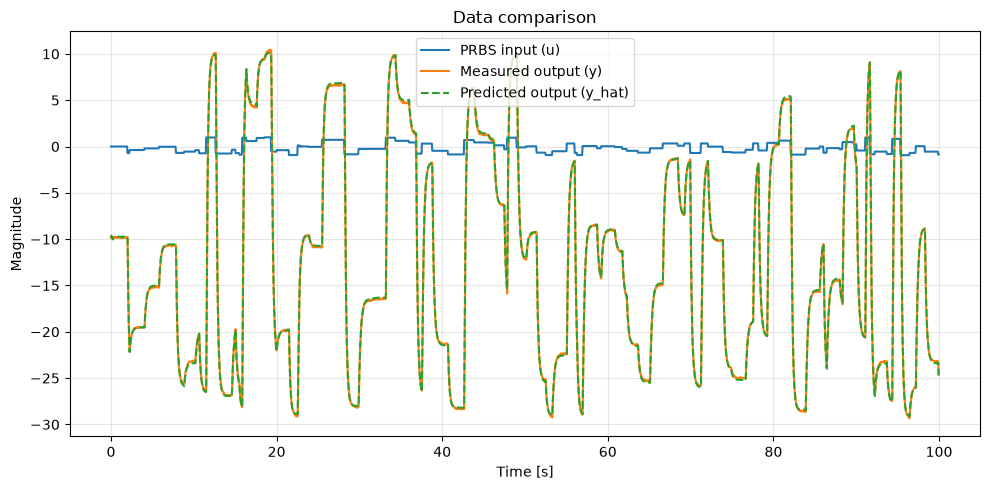
\includegraphics[
                width=0.92\textwidth,
                height=0.75\textheight,
                keepaspectratio
            ]{RNN1_results.png}
        \end{column}

    \end{columns}
\end{frame}